% title: One fixed-point feedback refinement
% description: With adj_iters set to one, output feedback enters the first step pullback. Its state feedback is accumulated with the original output feedback. A second step pullback uses the combined feedback to produce feedback for theta. Both pullbacks use the same returned state and theta. Feedback to the initial state is zero.
\documentclass[tikz,border=5pt]{standalone}
\usetikzlibrary{arrows.meta,calc,shapes.geometric}
\definecolor{numeric}{HTML}{4477AA}
\definecolor{textual}{HTML}{AA4499}

\tikzset{
    box/.style={draw, line width=0.8pt, minimum height=0.8cm,
                minimum width=1.8cm, inner sep=6pt, align=center},
    ir/.style={box},
    flow/.style={-{Stealth[length=5pt]}, line width=0.9pt},
    feedback/.style={flow, dashed},
    note/.style={font=\small, align=center},
    choice/.style={diamond, draw, line width=0.8pt,
                   aspect=2, inner sep=2pt, align=center},
}

\newcommand{\irframe}[2]{
    \draw[line width=0.8pt] #1 rectangle #2;
}

\newcommand{\transformarrow}[4][above]{
    \draw[flow] (#2) -- node[#1=6pt,note] {#4} (#3);
}

\begin{document}
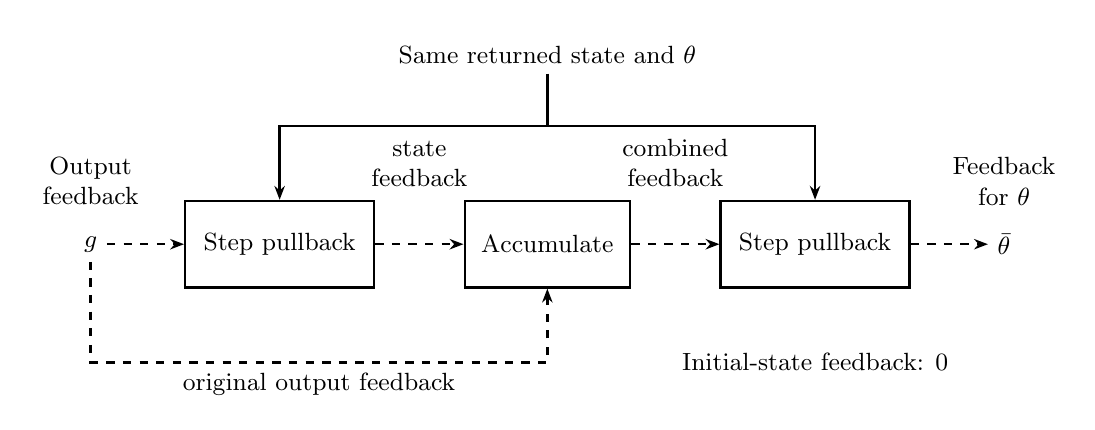
\begin{tikzpicture}[font=\small]
    \path[use as bounding box] (-6.6,-2.0) rectangle (6.6,2.75);

    \node (saved) at (0,2.4) {Same returned state and $\theta$};
    \node[box, minimum width=2.4cm, minimum height=1.1cm]
        (first) at (-3.4,0) {Step pullback};
    \node[box, minimum width=2.0cm, minimum height=1.1cm]
        (accum) at (0,0) {Accumulate};
    \node[box, minimum width=2.4cm, minimum height=1.1cm]
        (second) at (3.4,0) {Step pullback};

    \draw[line width=0.9pt] (saved.south) -- (0,1.5);
    \draw[flow] (0,1.5) -| (first.north);
    \draw[flow] (0,1.5) -| (second.north);

    \node (seed) at (-5.8,0) {$g$};
    \node[note] at (-5.8,0.8) {Output\\feedback};
    \node (thetafeedback) at (5.8,0) {$\bar{\theta}$};
    \node[note] at (5.8,0.8) {Feedback\\for $\theta$};
    \draw[feedback] (seed) -- (first);
    \draw[feedback] (first) -- node[above=17pt,note] {state\\feedback} (accum);
    \draw[feedback] (accum) -- node[above=17pt,note] {combined\\feedback} (second);
    \draw[feedback] (second) -- (thetafeedback);

    \draw[feedback] (seed.south) -- (-5.8,-1.5)
        -- node[below,note] {original output feedback} (0,-1.5) -- (accum.south);
    \node[note] at (3.4,-1.5) {Initial-state feedback: $0$};
\end{tikzpicture}
\end{document}
